%!TEX root = ../template.tex
%%%%%%%%%%%%%%%%%%%%%%%%%%%%%%%%%%%%%%%%%%%%%%%%%%%%%%%%%%%%%%%%%%%%
%% chapter5.tex
%% NOVA thesis document file
%%
%% Chapter with lots of dummy text
%%%%%%%%%%%%%%%%%%%%%%%%%%%%%%%%%%%%%%%%%%%%%%%%%%%%%%%%%%%%%%%%%%%%

\typeout{NT FILE chapter5.tex}%
\chapter{Implementation Details}
\label{cha:system_implementation}
This chapter begins in Section \ref{sec:communication} with an explanation of the implementation connecting Unity requests to the database.
The implementation process of all functionalities developed within the \gls{VE} is defined in Section \ref{sec:implementation}.
Then, the three fundamental techniques are described in detail in Section \ref{sec:techniques}.
Subsequently, Section \ref{sec:testing} clarifies the testing and debugging methodologies applied during the dissertation.
Finally, Section \ref{sec:impl_discussion} resumes the implementation process.

\section{Communication between Unity and Database}
\label{sec:communication}
This section describes the process of connecting Unity to the database. 
The workflow proceeds as follows: Unity sends requests to the backend, which then forwards them to the database and returns the requested data to Unity. 
The first subsection presents the endpoints required to retrieve the necessary data, while the subsequent subsection details the specific requests made in Unity for data visualization.

\subsection{\gls{API} Endpoints}

To retrieve information from the database for each object, requests are made to the repository layer. 
Two main \gls{API} endpoints were implemented for this purpose:

\begin{enumerate}
  \item \textbf{/GET (get-objects\_data)}
  \\Retrieves a list of object IDs by querying the \textbf{"object"} table. These IDs are used to populate the dropdown menu options in the \gls{UI}.

  \item \textbf{/GET (get-objects\_data/:id)}
  \\Fetches detailed information for a specific object based on its ID. This request is triggered when a user selects an object ID from the dropdown menu in the \gls{UI}
  Whenever the ID in the dropdown is changed, the system issues a new request for the corresponding ID, and the visualization panel and image gallery are updated accordingly.

    The representation of this endpoint is shown in Listing \ref{lst:api}. As illustrated in line 6, the query joins two tables, \textbf{"object"} and \textbf{"object\_intervention"}, to fetch simultaneously object data and images before and after interventions for display in the Image Gallery feature. 
    This SQL query enables the system to retrieve all necessary information with a single request after the user selects an object ID, thereby improving efficiency and reducing the need for multiple requests.

\end{enumerate}

\begin{lstlisting}[language=C++, caption={Example of defining an \gls{API} endpoint in Node.js.},label={lst:api},float]
  //GET endpoint that retrieves object data by ID
  app.get('/get-objects_data/:id', async (req, res) => {
    const id = req.params.id;

    try {
        // Query to the database: select all object data present in 'object' and 'object_intervention' tables by ID
        const result = await pool.query('SELECT * FROM object inner join object_intervention on object.id = object_intervention.object_id WHERE object.id = $1', [id]);
        res.json(result.rows[0]);
    } catch (error) {
        console.error(error);
        res.status(500).send('Server Error');
    }
});
\end{lstlisting}

\subsection{Unity requests to the Backend}
The \textbf{UnityWebRequest} class was used to send HTTP requests to the Node.js server, supporting both options retrieval (Section \ref{sec:options}) and object data retrieval (Section \ref{sec:data_retrieval}).

To acquire the desired data retrieval, only three data structures were required:  
\begin{enumerate}
    \item \textbf{Artifact} – representing an individual artefact and containing all attributes from the \texttt{artifact} table described in Chapter \ref{cha:system_design}, Section \ref{sec:database}.  
    \item \textbf{Dimensions} – a substructure of \textbf{Artifact}, storing three measurements: weight, height, and width.  
    \item \textbf{Artifact List} – a collection of \textbf{Artifact} structures to manage multiple objects retrieved from the database.  
\end{enumerate}
% The structures required to retrieve the desired object attributes are represented in Listing \ref{lst:structure}.

% \begin{lstlisting}[language=C++, caption={Artifact Structure to extract responses.}, label={lst:structure}]
% public class Dimensions
% {
%     public float height;
%     public float width;
%     public float weight;
% }

% public class Artifact
% {
%     public int id;
%     public int tomb_id;
%     public string name;
%     public string material;
%     public string glass_type;
%     public string shape;
%     public Dimensions dimensions;
%     public bool is_fragmented;
%     public bool has_pontil_mark;
%     public bool has_gold_fragments;
%     public string provenance;
%     public string general_description;
%     public string epoch;
%     public string[] paralels_url;
%     public string[] images_path_b_interv;
%     public string[] images_path_a_interv;
% }
% public class ArtifactList
% {
%     public List<Artifact> items;
% }
% \end{lstlisting}

\subsubsection{Dropdown Options Retrieval}
\label{sec:options}

This implementation retrieves all the IDs of the available artefacts, to fulfill the requirement of the user to view the desired object's textual and image information.  
The artefacts returned from the database are stored in a list structure, which is then iterated to populate the dropdown \texttt{options} list, as illustrated in Listing~\ref{lst:artifact_ids}.

\begin{lstlisting}[language=C++, caption={Method used to load artefact IDs and define as options in the Dropdown.}, label={lst:artifact_ids},float] 
      IEnumerator GetOptionsIds(string url)
    {
        // Send HTTP GET request to the given URL
        UnityWebRequest www = UnityWebRequest.Get(url);
        ...
        if (www.result == UnityWebRequest.Result.Success)
        {
            ...
            ArtifactList artifactList = JsonUtility.FromJson<ArtifactList>(wrappedJson);
            
            List<TMP_Dropdown.OptionData> options = new List<TMP_Dropdown.OptionData>();
            ...
            // Iterate through all artifacts and add their IDs to options List
            foreach (Artifact artifact in artifactList.items)
            {
                string id = artifact.id.ToString();
                options.Add(new TMP_Dropdown.OptionData("     " + id));
            }
            dropdown.AddOptions(options);
        }
        else{
            Debug.LogError("Error: " + www.error);
        }
    }
\end{lstlisting}


\subsubsection{Object Data Retrieval}
\label{sec:data_retrieval}
This method, shown in Listing \ref{lst:get_data}, retrieves all data of objects necessary to present in the \gls{VE}.  
It sends a \texttt{GET} request to obtain the complete information, including images before and after objects intervention.  

Additionally, textual data is retrieved. Once the request is successful, the JSON response is parsed into an \texttt{Artifact} object using Unity's \texttt{JsonUtility.FromJson<Artifact>()} method.  
From this structure, the following relevant fields are extracted: \emph{id}, \emph{name}, \emph{material}, \emph{epoch}, \emph{provenance}, and \emph{dimensions}.  
The \emph{dimensions} field is a nested JSON structure containing \emph{height}, \emph{width}, and \emph{weight}.  

Finally, a formatted string is created to display the object's details in the \gls{UI} panel functionality.

\begin{lstlisting}[language=C++,label={lst:get_data}, caption={Method used to load object data from the database},float]
      IEnumerator GetData(string url)
    {
        UnityWebRequest www = UnityWebRequest.Get(url);
        yield return www.SendWebRequest();

        if (www.result == UnityWebRequest.Result.Success)
        {
            artifact = JsonUtility.FromJson<Artifact>(www.downloadHandler.text);

            string displayText = "<b>Object Details:</b>\n\n";
            string material = artifact.material.Replace("{", "").Replace("}", "");

             displayText += $"ID: {artifact.id} | Name: {artifact.name} \nMaterial: {material} | Epoch: {artifact.epoch} \nProvenance: {artifact.provenance}" +
                         $"\nDimensions: {artifact.dimensions.height} x {artifact.dimensions.width} cm, Weight: {Mathf.Round(artifact.dimensions.weight * 10.0f) * 0.1f} g";

            resultText.text = displayText;
            GetImages(artifact.id, artifact.images_path_b_interv);
        }
        ...
    }
\end{lstlisting}


\section{Virtual Environment}
\label{sec:implementation}
The initial step was to place the \gls{2D} map on the ground plane, using the 1-meter default grid scale of Unity to ensure the precise real-world dimensions. With this in place, it was only necessary to adjust the scale of the funerary enclosure to match its position on the map. It is also important to mention that the two objects in the environment were carefully measured using virtual rules.

In the \gls{VE}, a set of functionalities was implemented. 
They are described in this section, in the following order: the Main Menu in Section \ref{sec:main_menu}, the Panel \gls{UI} in Section \ref{sec:panel_UI}, and Points of Interest in Section \ref{sec:points_interest}. 
Furthermore, funerary interaction is described in Section \ref{sec:funerary_interaction}, and navigation logic in Sections \ref{sec:user_navigation} and \ref{sec:tomb_logic}.

\subsection{Main Menu}
\label{sec:main_menu}

 \begin{figure}[h!]
    \centering
    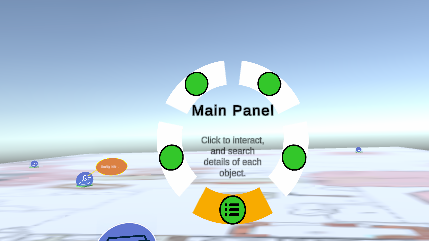
\includegraphics[width=0.7\linewidth]{Implementation/main_menu}
    \caption{Main Menu Interaction, with the option of the Main Panel selected.}
    \label{fig:main_menu}
\end{figure}

The main menu, displayed in Figure \ref{fig:main_menu}, was built with the support of the \textbf{SimplePieMenu} asset.
However, it was restructured and adapted for use with \gls{VR} controllers, since the original implementation was developed for Unity \gls{3D} without \gls{VR} handling.
The menu can be opened or closed with the trigger button of the right controller. The menu follows the user through the position of the right controller attributed in the "Follow\_Controller" script.
Additionally, to select an option, the user points at it with the ray and selects it using the right controller’s select button. To detect which menu option is being targeted, a \textbf{Raycast} operation is performed based on the current position of the right controller ray, as illustrated in Listing \ref{lst:menu_raycast}.

Currently, the menu contains only one functional option, represented by a menu icon. This option performs a single action: activating or deactivating the \textbf{Panel \gls{UI}} menu.


\begin{lstlisting}[language=C++, caption={Method used to acquire the position that was pointed at by the controller ray.}, label={lst:menu_raycast},float]
    public Vector2 GetPosition(Vector2 anchoredPosition, Transform controllerTransform)
    {
        // Create a ray starting from the controller's position, pointing forward
        Ray ray = new Ray(controllerTransform.position, controllerTransform.forward);
        /Ray to detects collisions with the main menu
        if (Physics.Raycast(ray, out RaycastHit hit, 50f, LayerMask.GetMask("Default")))
        {
            Vector3 screenPoint = Camera.main.WorldToScreenPoint(hit.point);
            
            // Return the point relative to the center of the screen
            return new Vector2(
                screenPoint.x - Screen.width / 2f,
                screenPoint.y - Screen.height / 2f);
        }
        return Vector2.zero;
    }
\end{lstlisting}



\subsection{Panel \gls{UI}}
\label{sec:panel_UI}
\begin{figure}[h!]
    \centering
    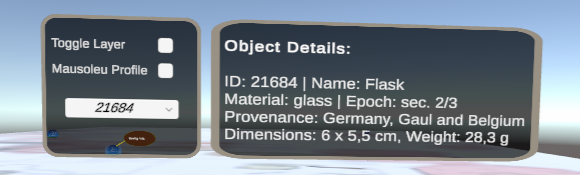
\includegraphics[width=0.8\linewidth]{Implementation/main_panel}
    \caption{Panel \gls{UI} Interaction.}
    \label{fig:main_panel}    
\end{figure}

The \gls{UI} includes a canvas where users can interact with and explore object data, as shown in the left panel of Figure \ref{fig:main_panel}. 

In this example, the object ID selected from the dropdown menu is "21684," and the textual data associated with this object is displayed in the right panel. 
This panel is initially empty and populates with the relevant object details after a selection is made. 

The \gls{UI} contains three interactive elements: the "Toggle Layer" and "Mausoleum Profile" checkboxes, and the "Dropdown Menu".

 \begin{figure}[h!]
    \centering
    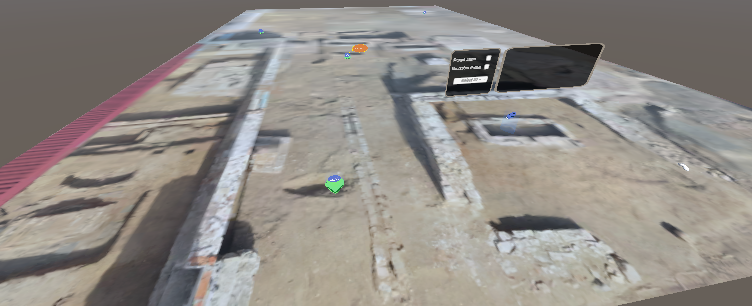
\includegraphics[width=0.8\linewidth]{Implementation/layer}
    \caption{Toggle Layer to a photo of the Site Occidental part.}
    \label{fig:toggle_layer}    
\end{figure}


 \begin{figure}[h!]
    \centering
    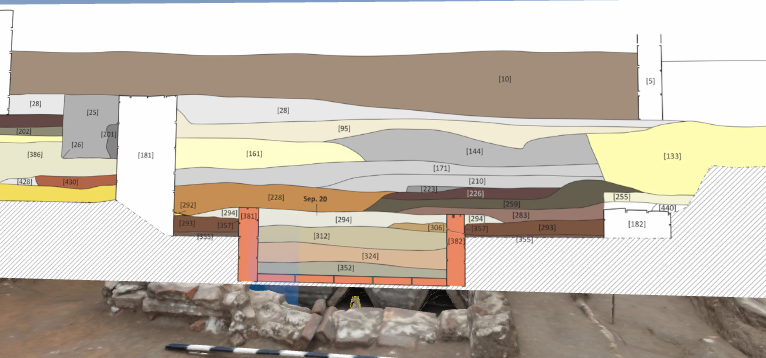
\includegraphics[width=0.8\linewidth]{Implementation/mausoleum_profile}
    \caption{Funerary Enclosure Profile constructions layer view.}
    \label{fig:mausoleum_profile}    
\end{figure}

The first element, \textbf{Toggle Layer}, is a checkbox that controls the visibility of the ground plane.
By default, the base plan is represented by a partial drawing of this archaeological site, which includes the burial enclosure under study. 
When the user activates the checkbox, the plan switches to a photograph of the actual site, offering a more realistic view and a stronger sense of presence. 
This feature is illustrated in Figure \ref{fig:toggle_layer}.
The user can at any time toggle the view in the checkbox to view the pretended plan.

The second element, the \textbf{Funerary Enclosure Profile}, demonstrated in Figure \ref{fig:mausoleum_profile}, works similarly. However, in this case, it opens a profile image of the mausoleum wall, displaying the different material types and layers of construction.

The third element, the \textbf{Dropdown Menu}, allows the user to select an object by its identification number (ID).
Once selected, the corresponding textual data and intervention images (Image Gallery) are retrieved from the database.
The Image Gallery is displayed on the left, while the right side presents the textual data corresponding to the selected Object ID.

\subsubsection{Image Gallery}
\label{sec:image_gallery}

\begin{figure}[h!]
    \centering
    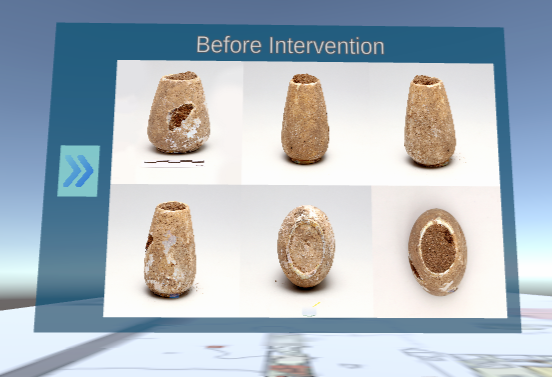
\includegraphics[width=0.7\textwidth]{Implementation/images_gallery}
    \caption{Image Gallery with object images before intervention.}
    \label{fig:image_gallery}
\end{figure}

The image gallery, as mentioned, is activated upon object selection. 
This gallery displays images of the object before and after intervention. 
Users can switch between these states by hovering the controller ray over the gallery arrow. 
In this manner, they can view the images of a concrete object, compare the visual differences, and acquire a clearer understanding of the intervention's impact on each object.

The implementation was made through a \texttt{GetImages} method that iterates over the array of image paths retrieved from the "object\_intervention" table. The array passed to this method may be either "images\_path\_b\_interv", containing the object images before intervention, or "images\_path\_a\_interv", after the intervention.
For each image, a component is created and positioned appropriately within the gallery.
The process is presented in Listing \ref{lst:artefacts_images}.

\begin{lstlisting}[language=C++, caption={Method used to load artefact images and to display them in the Images Gallery.}, label={lst:artefacts_images},float]
      private void GetImages(int id, string[] images_path)
    {
        if (images_path.Length != 0)
        {
            changeView.SetActive(true);
            for (int x = 0; x < images_path.Length; x++)
            {
                var imagePath = images_path[x];

                if (x > images_path.Length / 2) {height = 0;}
                else if (x == images_path.Length / 2) { x_pos = 1.5f; height = 0; }
                else { height = 1; }

                Sprite sprite = Resources.Load<Sprite>("Images/" + imagePath);
                if (sprite != null)
                {
                    GameObject newImgObj = new GameObject("Image_" + imagePath, typeof(RectTransform), typeof(CanvasRenderer), typeof(Image));
                    newImgObj.transform.SetParent(imageParent, false);

                    RectTransform rectTransform = newImgObj.GetComponent<RectTransform>();
                    rectTransform.sizeDelta = new Vector2(1, 1);
                    rectTransform.localPosition = new Vector3(x_pos++, height, 0);

                    Image imgComponent = newImgObj.GetComponent<Image>();
                    imgComponent.sprite = sprite;
                }
                ...
            }
            x_pos = 1.5f;
        }
        else
        {
            Debug.LogWarning("Couldn't load Images for Object ID" + id);
        }
    }
\end{lstlisting}

\subsection{Points of Interest}
\label{sec:points_interest}

\begin{figure}[h!]
    \centering
    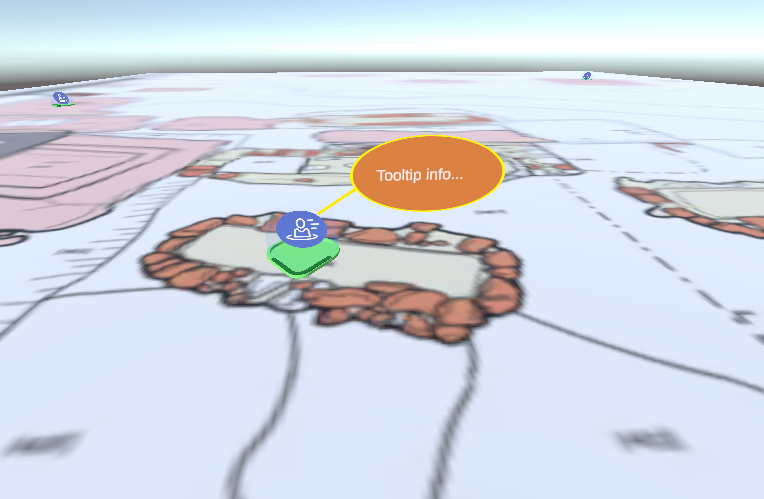
\includegraphics[width=0.7\textwidth]{Implementation/anchor_with_tool_tip}
    \caption{Exemplified point of interest with an aggregated tooltip.}
    \label{fig:points_interest}
\end{figure}

Diverse points of interest were placed in key areas across the plane.

Users can teleport directly to a point of interest by selecting a blue anchor (implemented with the default \emph{Teleportation Anchor} component) within the plan. These points are designed to draw the user’s attention to notable features or artefacts, with the most relevant point for the current study located inside the tomb within the funerary enclosure.
Figure \ref{fig:points_interest} illustrates one of these anchors.

In the future, the idea is to expand to other points and create interactive features as the \gls{3D} funerary enclosure model. 

\subsection{Object Interaction}
\label{sec:object_interact}
This section describes object interaction, starting with the Slider in Section \ref{sec:object_slider}, the Outline in Section \ref{sec:object_outline}, and Grab and Release in Section \ref{sec:object_interaction}

\subsubsection{Object Slider}
\label{sec:object_slider}

 \begin{figure}[h!]
    \centering
    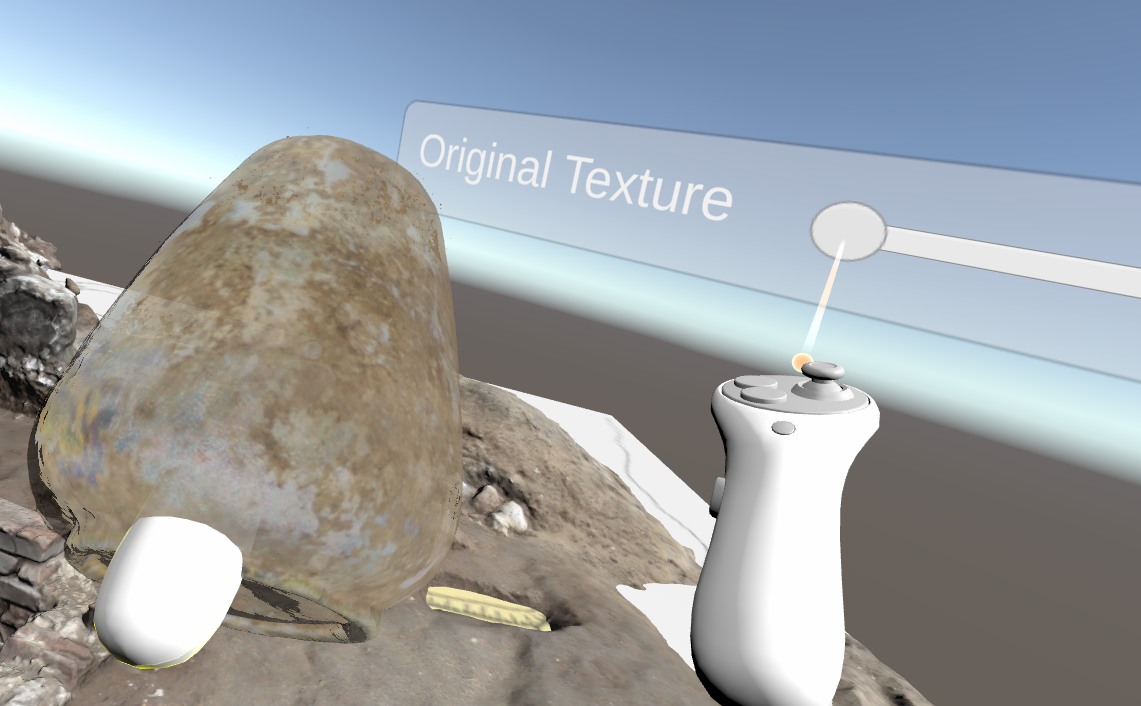
\includegraphics[width=0.8\linewidth]{Implementation/grab_object}
    \caption{Object Slider Interaction.}
    \label{fig:object_slider}
\end{figure}

The Object Slider was designed as an interactive feature within the \gls{VE}, allowing users to visualize an object's transformation over time, from its original condition to its current, restored state. 

This functionality is illustrated in Figure \ref{fig:object_slider}, where the user holds the object with the left controller while manipulating the slider, named “Original Texture,” with the right controller. 
The texture initially displayed corresponds to the post-excavation state, and as the user moves the slider to the right, it gradually transitions to the original glass texture.
The goal was to provide an immersive experience, creating the sensation of traveling back in time to observe the physical changes the object has undergone throughout the years.

Several experimental approaches were conducted to achieve this effect, focusing on shader development.
Two main approaches were explored, as described below:

The first attempt involved creating a shader that utilized a single texture input, specifically the texture of the object after restoration. A white color was used to control the alpha (transparency) values, and the transition effect was managed using a linear interpolation (lerp) function. This shader was developed using Unity’s Shader Graph, which provided a visual, node-based interface for building the transition logic.


The final solution involved a more advanced shader, written in Unity High-Level Shader Language (HLSL) for the Universal Render Pipeline (URP)\footnote{\url{https://docs.unity3d.com/Manual/urp/writing-custom-shaders-urp.html}}. 
This approach provided more control over the material's appearance compared to Unity's built-in shaders.
The shader was constructed using key URP shader libraries, including those for lighting and shading calculations\footnote{\url{https://docs.unity3d.com/Packages/com.unity.render-pipelines.universal@14.0/manual/use-built-in-shader-methods-lighting.html}}
, reflection probes\footnote{\url{https://docs.unity3d.com/Manual/urp/use-built-in-shader-methods-indirect-lighting.html}}
, shadow integration\footnote{\url{https://docs.unity3d.com/6000.1/Documentation/Manual/urp/use-built-in-shader-methods-shadows.html}}
, camera operations\footnote{\url{https://docs.unity3d.com/Manual/urp/use-built-in-shader-methods-camera.html}}
, and transformations\footnote{\url{https://docs.unity3d.com/Manual/urp/use-built-in-shader-methods-transformations.html}}.
%https://docs.unity3d.com/Manual/urp/use-built-in-shader-methods.html

This version accepted two texture inputs: the original appearance of the object (input variable \texttt{\_DecayTex}) and its current state (input variable \texttt{\_RestoredTex}).
Besides the texture inputs, the shader provides the following adjustable material properties: \emph{Blend Factor}, \emph{Smoothness}, \emph{Fresnel Power}, \emph{Specular Color}, and \emph{Reflection Intensity}, enabling precise control over how the textures blend and the visual appearance of the material. 
These properties can be modified directly through the Unity Inspector.

A \textbf{Lerp function}\footnote{\url{https://docs.unity3d.com/6000.2/Documentation/ScriptReference/Vector3.Lerp.html}} is a methodology that performs a linear interpolation between two values, based on an interpolation factor.
In this case, it was used to interpolate between the two textures, considering their \texttt{Albedo}, \texttt{Alpha}, and \texttt{Smoothness} attributes, as shown in Listing \ref{lst:shader_blend}. 
In this case, the interpolant factor is \emph{\_BlendFactor}, the input value that changes when the user moves the slider bar.

To enhance realism, additional lighting and reflection techniques were integrated into the shader, including 
the \textbf{Fresnel Effect}\footnote{\url{https://docs.unity3d.com/Packages/com.unity.shadergraph@6.9/manual/Fresnel-Effect-Node.html}} to model light behaviour based on the angle between the surface normal (\texttt{normalWS}) and the view direction (\texttt{viewDirWS}), 
and adjustments to \textbf{specular}, \textbf{diffuse}, and \textbf{environment lighting} properties. 
These calculations were performed independently for each component, as illustrated in Listing~\ref{lst:lighting_glass}, before being aggregated into the final \texttt{finalColor}. 
This shader enabled a more faithful representation of the object's original appearance.

\begin{lstlisting}[language=HLSL, caption={Partial Fragment shader for blending original and restored textures.}, label={lst:shader_blend},float]
        half4 frag(Varyings IN) : SV_Target
        {
            half4 decayAlbedo = SAMPLE_TEXTURE2D(_DecayTex, sampler_DecayTex, IN.uv);
            half4 restoredAlbedo = SAMPLE_TEXTURE2D(_RestoredTex, sampler_RestoredTex, IN.uv);

            float3 normalWS = normalize(IN.worldNormal);
            float3 viewDirWS = normalize(IN.viewDirWS);

            float fresnel = CalculateFresnel(normalWS, viewDirWS, _FresnelPower);

            half3 finalAlbedo = lerp(decayAlbedo.rgb, restoredAlbedo.rgb, _BlendFactor);
            half finalAlpha = lerp(decayAlbedo.a, restoredAlbedo.a, _BlendFactor);
            half finalSmoothness = lerp(_GlassSmoothness, _RestoredSmoothness, _BlendFactor);
            ... Populate Data...
            
            half3 glasslitColor = CalculateGlassLighting(surfaceData, inputData, fresnel);            
            half enhancedAlpha = lerp(finalAlpha, finalAlpha * 0.5, fresnel * 0.5);
            
            return half4(glasslitColor, enhancedAlpha);
        }
\end{lstlisting}


\begin{lstlisting}[language=C++, caption={Lighting Glass Texture Partial Calculation.}, label={lst:lighting_glass},float]
  float3 CalculateGlassLighting(SurfaceData surfaceData, InputData inputData, float fresnel)
  {
      Light mainLight = GetMainLight(inputData.shadowCoord, inputData.positionWS, inputData.shadowMask);
      ...
      float3 specular = specularTerm * mainLight.color * _SpecularColor.rgb * surfaceData.smoothness;
      ...
      float3 diffuse = lerp((surfaceData.albedo * mainLight.color * NdotL * 0.1),surfaceData.albedo, _BlendFactor);
      ...     
      float3 environmentReflection = GlossyEnvironmentReflection(reflectionVector, 
          inputData.positionWS, surfaceData.smoothness, 1.0) * _ReflectionIntensity;

      float3 finalColor = diffuse + (specular + environmentReflection * fresnel);
      
      return finalColor;
  }
\end{lstlisting}

\subsubsection{Object Outline}
\label{sec:object_outline}

 \begin{figure}[h!]
    \centering
    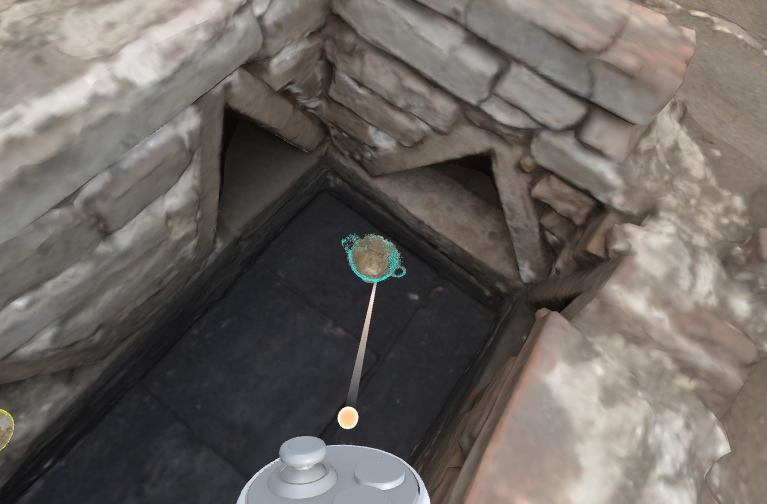
\includegraphics[width=0.8\linewidth]{Implementation/outline_object}
    \caption{Outline effect applied when an object is hited with the controller ray.}
    \label{fig:outline_object}    
\end{figure}


This functionality was implemented to improve the visibility of objects within the tomb and to distinguish them from the surrounding funerary ground.  
It essentially consists of an outline shader and a complementary script that manages its parameters. 
The shader highlights objects when targeted with the controller ray, as illustrated in Figure~\ref{fig:outline_object}

The shader includes the following input parameters: \emph{Outline Color}, \emph{Outline Width}, \emph{Outline Power}, and \emph{Outline Softness}.  
Similar to the shader described for the Object Slider functionality in Section~\ref{sec:object_slider}, this shader also relies on the Fresnel effect to control outline intensity and appearance.  

The rendering of each object includes two materials: a primary material representing its texture and a secondary material responsible for the outline effect.
When the user points at the object, the parameter \texttt{OutlineColor} is switched from yellow to blue. But if the object is not being grabbed (\texttt{if(!select)}), the outline disappears. 
This behavior is handled through hover events, as shown in Listing~\ref{lst:outline_color}. 
By accessing the second material of the object via \texttt{meshRenderer.materials[1]}, the shader updates the outline color.  

The fragment shader logic for the glowing outline is presented in Listing~\ref{lst:outline_effect}. 
It computes the Fresnel term with the Outline Power attribute, and applies a \texttt{smoothstep()} to achieve a soft personalized outline.  
This mechanism ensures that the objects are easily identifiable. 

\begin{lstlisting}[language=C++, caption={Partial class with Outline Color changed when the object is Hovered.}, label={lst:outline_color},float]
    public class GlowingObject : MonoBehaviour
{
    private MeshRenderer meshRenderer;
    private bool select = false;
    Color Yellow = new Color(65, 65, 0, 1);
    Color Blue = new Color(0, 59, 49, 1);
    ...
    public void OnHoverEnter()
    {
        meshRenderer.materials[1].SetColor("_OutlineColor", Blue);
    }

    public void OnHoverExit()
    {
        if(!select)
            meshRenderer.materials[1].SetColor("_OutlineColor", Yellow);
    }
    ...
}
\end{lstlisting}


\begin{lstlisting}[language=HLSL, caption={Partial Fragment shader for creating an outline effect to the object.}, label={lst:outline_effect},float]
        float4 frag(v2f i) : SV_Target
        {
            float3 N = normalize(i.normalWS);
            float3 V = normalize(i.viewDirWS);

            float fresnel = pow(1.0 - saturate(dot(N, V)), _OutlinePower);

            float edge1 = 1.0 - _OutlineWidth;
            float edge2 = edge1 + _OutlineSoftness;
            float outlineFactor = smoothstep(edge1, edge2, fresnel);

            return _OutlineColor * outlineFactor;
        }
\end{lstlisting}

\subsubsection{Grab and Release Object}
\label{sec:object_interaction}

The artefacts can be grabbed with the lateral button of the controllers.
When the object is grabbed or released, the corresponding event in Listing~\ref{lst:grab_release} is triggered.  

The proximity of the controller's ray to the object determines how close the object appears to the user's view. 
Releasing the object is achieved simply by releasing the button.  
Small objects are automatically zoomed when hovered over or grabbed (operation \texttt{transform.localScale = zoomScale}), improving clarity and visibility during interaction.

Additionally, two other behaviors are implemented. 
The colliders that might interfere during grabbing are reactivated upon release, except when the user is inside the tomb, in which case a coroutine (\texttt{StartCoroutine}) is executed.
During \texttt{OnGrab}, and as illustrated in Figure \ref{fig:object_slider}, the object slider is repositioned depending on whether the object is grabbed with the left or right controller, controlled by the \texttt{CompareTag} method.

\begin{lstlisting}[language=C++, caption={Partial Fragment of objects onGrab and onRelease events.}, label={lst:grab_release},float]
     
    private void OnGrab(SelectEnterEventArgs args)
    {
        transform.localScale = zoomScale;
        args.interactableObject.colliders.ForEach(collider => { collider.enabled = false; });
        ...
        var interactor = args.interactorObject.transform;
        if (interactor.CompareTag("left")) 
        {
            follow.targetOffset = new Vector3(sliderRightxPos, follow.targetOffset.y, follow.targetOffset.z);
        }
        else if (interactor.CompareTag("right")) 
        {
            follow.targetOffset = new Vector3(sliderLeftxPos, follow.targetOffset.y, follow.targetOffset.z);
        }
    }

    private void OnRelease(SelectExitEventArgs args)
    {
        transform.localScale = originalScale;
        args.interactableObject.colliders.ForEach(collider => { collider.enabled = true; });
        ...
        if (r.isInsideTomb)
        {
            StartCoroutine(DisableColliderRoutine(5f));
        }
        ...
    }
\end{lstlisting}


\subsection{Funerary Enclosure Interaction}
\label{sec:funerary_interaction}

 \begin{figure}[h!]
    \centering
    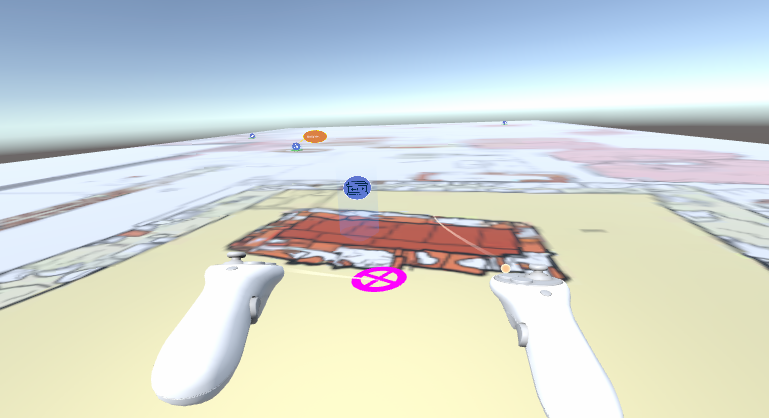
\includegraphics[width=0.8\linewidth]{Implementation/default_plan_with_reticle}
    \caption{Funerary Enclosure Activation Reticle in the default ground plan.}
    \label{fig:funerary_interaction}    
\end{figure}

The system provides the possibility to activate or deactivate the \gls{3D} model of the funerary enclosure.
This functionality is triggered using the trigger button of the left command. When the user points to the funerary enclosure area in the map, a purple reticle appears, indicating that the enclosure can be activated, as illustrated in Figure \ref{fig:funerary_interaction}. This interaction can be performed at any point during the experience.

To ensure realism, the funerary enclosure is implemented with a default \emph{Mesh Collider} combined with an aggregated \emph{Rigidbody}. This configuration prevents the user from crossing the enclosure walls and accurately reproduces the surface levels of the original structure, thereby enhancing the immersive experience.

An exception occurs when the user is inside the tomb. In this case, the funerary enclosure collider is temporarily disabled, allowing the user to descend naturally to the ground without obstruction. Once the user exits the tomb, the collider is restored to maintain consistent collision detection.

\subsection{User Navigation}
\label{sec:user_navigation}

The user can navigate in the environment with the controllers. 
These allow two modes of movement: continuous walking, which simulates real-world locomotion, and teleportation, providing a faster way to reposition within the scene.

There are two types of teleportation available in the environment. The first allows the user to teleport freely to any position on the environment’s ground plane (default \emph{Teleportation Area} component). The second restricts teleportation to specific points of interest, marked with blue icons (anchors).

In addition to locomotion, users can switch their perspective inside the environment, using the controllers, moving laterally with the right joystick.
Both continuous movement and snap turning can also be performed physically, without controllers, within the limits of the real-world space.

The overall movement system is managed by the \emph{Character Controller} component, which also ensures accurate collision detection. In particular, the collider associated with the user interacts with the collider of the funerary enclosure, preventing the user from passing through walls and thereby preserving realism in the experience.

Further refinements and a dynamic management of movement behavior were introduced in the script "CustomMovement", where two key methods were implemented within Unity’s default \texttt{Update()} function.
The first method (Listing \ref{lst:recenter}) continuously updates the center of the character controller to reflect the user’s current position during locomotion. 
The second (Listing \ref{lst:gravity}) manages custom movement behaviors by dynamically controlling gravity with \texttt{velocityY}. 
Depending on the context, gravity may either be applied or disabled. When active, it influences the user’s velocity over time, and its intensity can be adjusted dynamically (\texttt{gravityMultiplier}).

\begin{lstlisting}[language=C++, caption={Recenter user position method.}, label={lst:recenter},float]
void UpdateCharacterHeight()
{
    Vector3 center = transform.InverseTransformPoint(origin.Camera.transform.position);
    character.center = new Vector3(center.x, center.y, center.z);
}
\end{lstlisting}


\begin{lstlisting}[language=C++, caption={Apply costum gravity method.}, label={lst:gravity},float]
  private void ApplyCustomGravity()
  {
      Vector3 current = origin.Camera.transform.localPosition;
      Vector3 delta = current - previousCamPos;  // movement since last frame
      velocityY = delta.y;

      if (character.isGrounded) //check if user is currently touching the ground plan
      {
          velocityY = 0f;
      }
      else
      {
          velocityY += Physics.gravity.y * Time.deltaTime* gravityMultiplier; // Apply custom gravity 
      }
      Vector3 move = new Vector3(delta.x, velocityY, delta.z);
      character.Move(move * Time.deltaTime); // update user movement
      previousCamPos = current; // update previous camera position for next frame
  }
\end{lstlisting}

\subsection{Tomb Navigation Logic}
\label{sec:tomb_logic}

 \begin{figure}[h!]
    \centering
    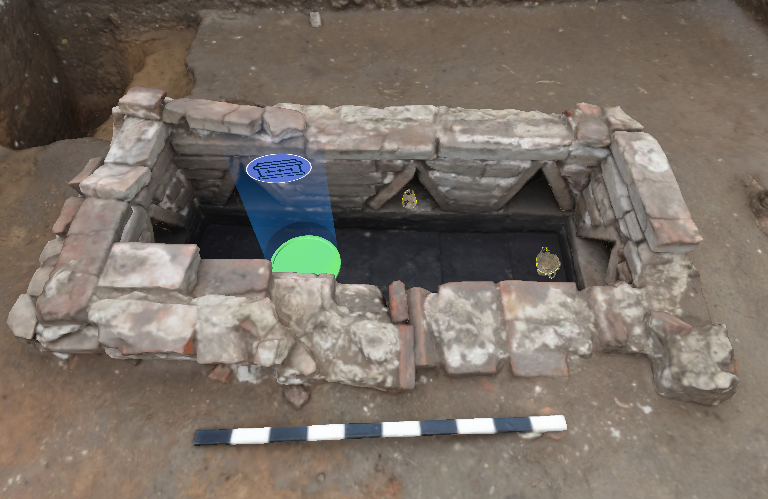
\includegraphics[width=0.8\linewidth]{Implementation/tomb_outside}
    \caption{Tomb Exterior View with blue anchor inside.}
    \label{fig:tomb_outside}    
\end{figure}

 \begin{figure}[h!]
    \centering
    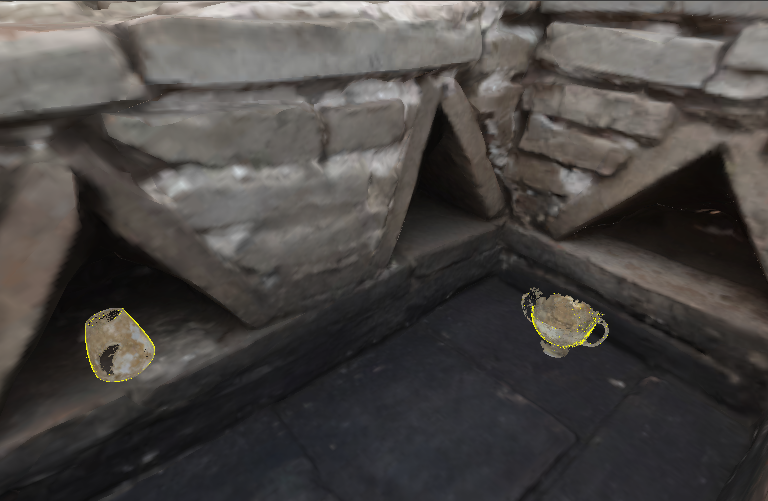
\includegraphics[width=0.8\linewidth]{Implementation/tomb_inside}
    \caption{Tomb Interior View with Objects positioned.}
    \label{fig:tomb_inside}    
\end{figure}

To access the tomb, the user may either walk in continuous movement toward its interior or use teleportation by clicking on the blue anchor located in that area.
Upon entering, the user will have a view similar to the one shown in Figure \ref{fig:tomb_inside}.
The tomb contains triangular areas, that was the place where the majority of the objects were discovered. 
It's important to note that the artefacts are presented in the exact positions in which they were found during the excavations.
During the dissertation process, different techniques were implemented and tested to address navigation and visualization challenges inside the tomb.

\subsection*{Plan Removal}

The first approach used a collider placed inside the tomb. When the user collided with it, the ground plane was removed, revealing the full interior of the tomb.

This, in the end, caused conflicts because the interior collider overlapped with the collider responsible for activating the funerary enclosure.

To handle this issue, the limits of the tomb (coordinates x, y, and z) were defined manually. With this method, shown in Listing \ref{lst:plan_removal}, the plane disappears when the user enters that space and reappears once the user exits it.
In Figure \ref{fig:tomb_outside}, the outside view of the tomb is depicted. As illustrated, the plane is disabled, providing full visibility of the tomb’s interior.


\begin{lstlisting}[language=C++, caption={Plan Removal approach in Update method().}, label={lst:plan_removal},float]
 void Update()
 {
     if (excavation_model.activeSelf) //check if funerary model is active
     {
         if (camara.position.x >= x_min && camara.position.x <= x_max && camara.position.z <= z_max && camara.position.z >= z_min && camara.position.y <= y_max && camara.position.y >= y_min)
         {
            if(toggle_UI.firstactive) //deactivate the plan if inside the tomb area
                 plane.SetActive(false);
            else plane2.SetActive(false);

            if(camara.position.y <= plane.transform.position.y + 0.4f) 
                 mausoleu.SetActive(false); //disable mausoleum collider so the user can fall inside the tomb without colliding
             isInsideTomb = true;
         }
         else
         {
             if (toggle_UI.firstactive) //reactivate the plan if outside the tomb area
                 plane.SetActive(true);
             else
                 plane2.SetActive(true);
             isInsideTomb = false;
             mausoleu.SetActive(true); //reactivate mausoleum collider 
         }
     }
 }
\end{lstlisting}
\subsection*{Vertical Descend}

Another challenge was ensuring that users could navigate naturally within the tomb while maintaining clear visibility of objects and architectural details inside. Standard gravity alone was insufficient, as it did not allow reliable interaction with objects located in triangular areas.
To address this, the "TombNavigation" script was developed, introducing controlled vertical displacement along the y-axis.

Initially, a Raycasting approach was tested, directing rays toward the front and the floor of the tomb. When a collision was detected, the user’s position was adjusted and lowered by a few centimeters. Although functional, this method is unreliable, as it heavily depends on the user’s viewing direction, extracted from the camera position.

The final implementation instead defined the tomb interior using axis-based boundaries (x, y, and z coordinates). 
When the user entered this delimited area, they were automatically replaced downward with the \texttt{new\_y} factor. Upon exiting, the user’s position was restored to its correct height (\texttt{camPosbefore}), ensuring they did not remain unnaturally below the expected level. 
This approach, respresented in Listing \ref{lst:vertical_descend} allows the user to enter and exit the tomb by simply walking.

During development, two alternative exit mechanisms, a block and a ladder, were added. However, these were later deactivated, as they were unnecessary with the finalized gravity-based solution and occupied additional space in the relatively small tomb environment. Nevertheless, both alternatives remain available for reactivation if required in the future.

\begin{lstlisting}[language=C++, caption={Vertical Descend approach in Update method().}, label={lst:vertical_descend},float]
void Update()
{
    var camara = Camera.main.transform;
    if (!isInside && cam.transform.localPosition.y != new_y)
    {
        camPosbefore = cam.transform.localPosition; //position before entering the tomb
    }
    if (!plane.activeSelf && camara.position.x >= x_min && camara.position.x <= x_max && camara.position.z <= z_max && camara.position.z >= z_min && camara.position.y <= y_max && camara.position.y >= y_min) //check if position inside the tomb
    {
        isInside = true;
        mausoleu_collider.SetActive(false); //deactivate funerary collider
        cam.transform.localPosition = new Vector3(cam.transform.localPosition.x, new_y, cam.transform.localPosition.z); //user replaced to a lower position
    }
    else
    {
        isInside = false;
        mausoleu_collider.SetActive(true);
        cam.transform.localPosition = camPosbefore;
    }
}

\end{lstlisting}
%Essential Stages/Steps
\section{Key Techniques}
\label{sec:techniques}
This section describes the main techniques implemented during the development process. 
The first two techniques focus on optimizing \gls{UX} and improving system performance by significantly reducing the complexity of the funerary model, while preserving essential detail. 
The last two techniques detail the methodologies used to generate the glass material and the funerary \gls{3D} model.
\subsection{Light Technique}
There is a main directional light that illuminates the entire environment, simulating reality. 
However, it was understood that depending on the angle, the user might see the tomb and objects as black due to shadows. To address this, a secondary point light was added that follows the user, so the user can view the tomb with clarity and have a good visibility while navigating in the environment.

\subsection{Funerary Enclosure Model Reduction}
The resolution of the burial site model was significantly reduced in \emph{Agisoft Metashape} software through the "Decimate Model" property.
This adjustment was necessary due to warnings of potential collision issues arising from the model's size of over 2 million triangles. 
Therefore, the number of faces was reduced from 1.9 million to approximately 100 thousand, preserving the essential level of detail while improving efficiency.

\subsection{Generating the Glass Texture}
\label{sec:glass_texture}
The process of generating the glass texture consisted of two phases.  

First, the material was modeled in Blender using a node-based shader structure. The desired glass effect was achieved by combining the \texttt{Glossy BSDF} and \texttt{Refraction BSDF} nodes. It also received a \texttt{Fresnel} node as input\footnote{\url{https://docs.blender.org/manual/en/latest/render/shader_nodes/index.html}}. This structure is represented in Figure~\ref{fig:glass_texture}.  

After having the node structure, a UV unwrapping\footnote {\url{https://docs.blender.org/manual/en/latest/modeling/meshes/uv/unwrapping/}} was made to prepare the \gls{3D} object surface for texture mapping, process illustrated in Figure \ref{fig:uv_process}.
 Finally, a baking process\footnote{\url{https://docs.blender.org/manual/en/latest/render/cycles/baking.html}} was performed using the Cycles render engine.
With these materials, a "Combined" texture was baked and imported to Unity as a .png file.

 \begin{figure}[h!]
    \centering
    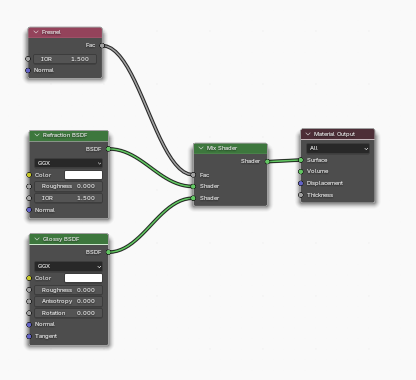
\includegraphics[width=0.8\linewidth]{Implementation/Glass_texture}
    \caption{Glass Material Nodes Blender.}
    \label{fig:glass_texture}    
\end{figure}


\begin{figure}[h!]
    \centering
    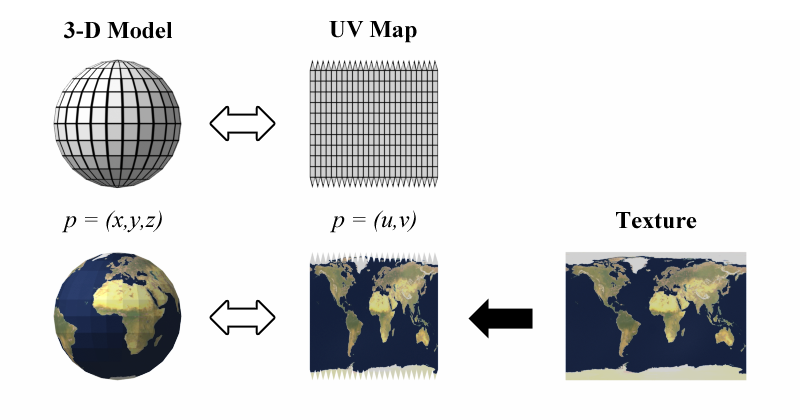
\includegraphics[width=0.8\textwidth]{Implementation/UVMapping}
    \caption{UV unwrapping process with corresponding mapped texture.}
    \label{fig:uv_process}
\end{figure}


In Unity, one \textbf{Reflection Probe} for each object was added to simulate the environment's reflection on the glass surface.
Additionally, the four attributes \emph{\_GlassSmoothness}, \emph{\_FresnelPower}, \emph{\_SpecularColor}, and \emph{\_ReflectionIntensity}, used in the slider shader in Section \ref{sec:object_slider}, can be adjusted to control the pretended reflections in the glass.
The final glass texture exemplifying one object is illustrated in Figure \ref{fig:glass1}.

\begin{figure}[h!]
    \centering
    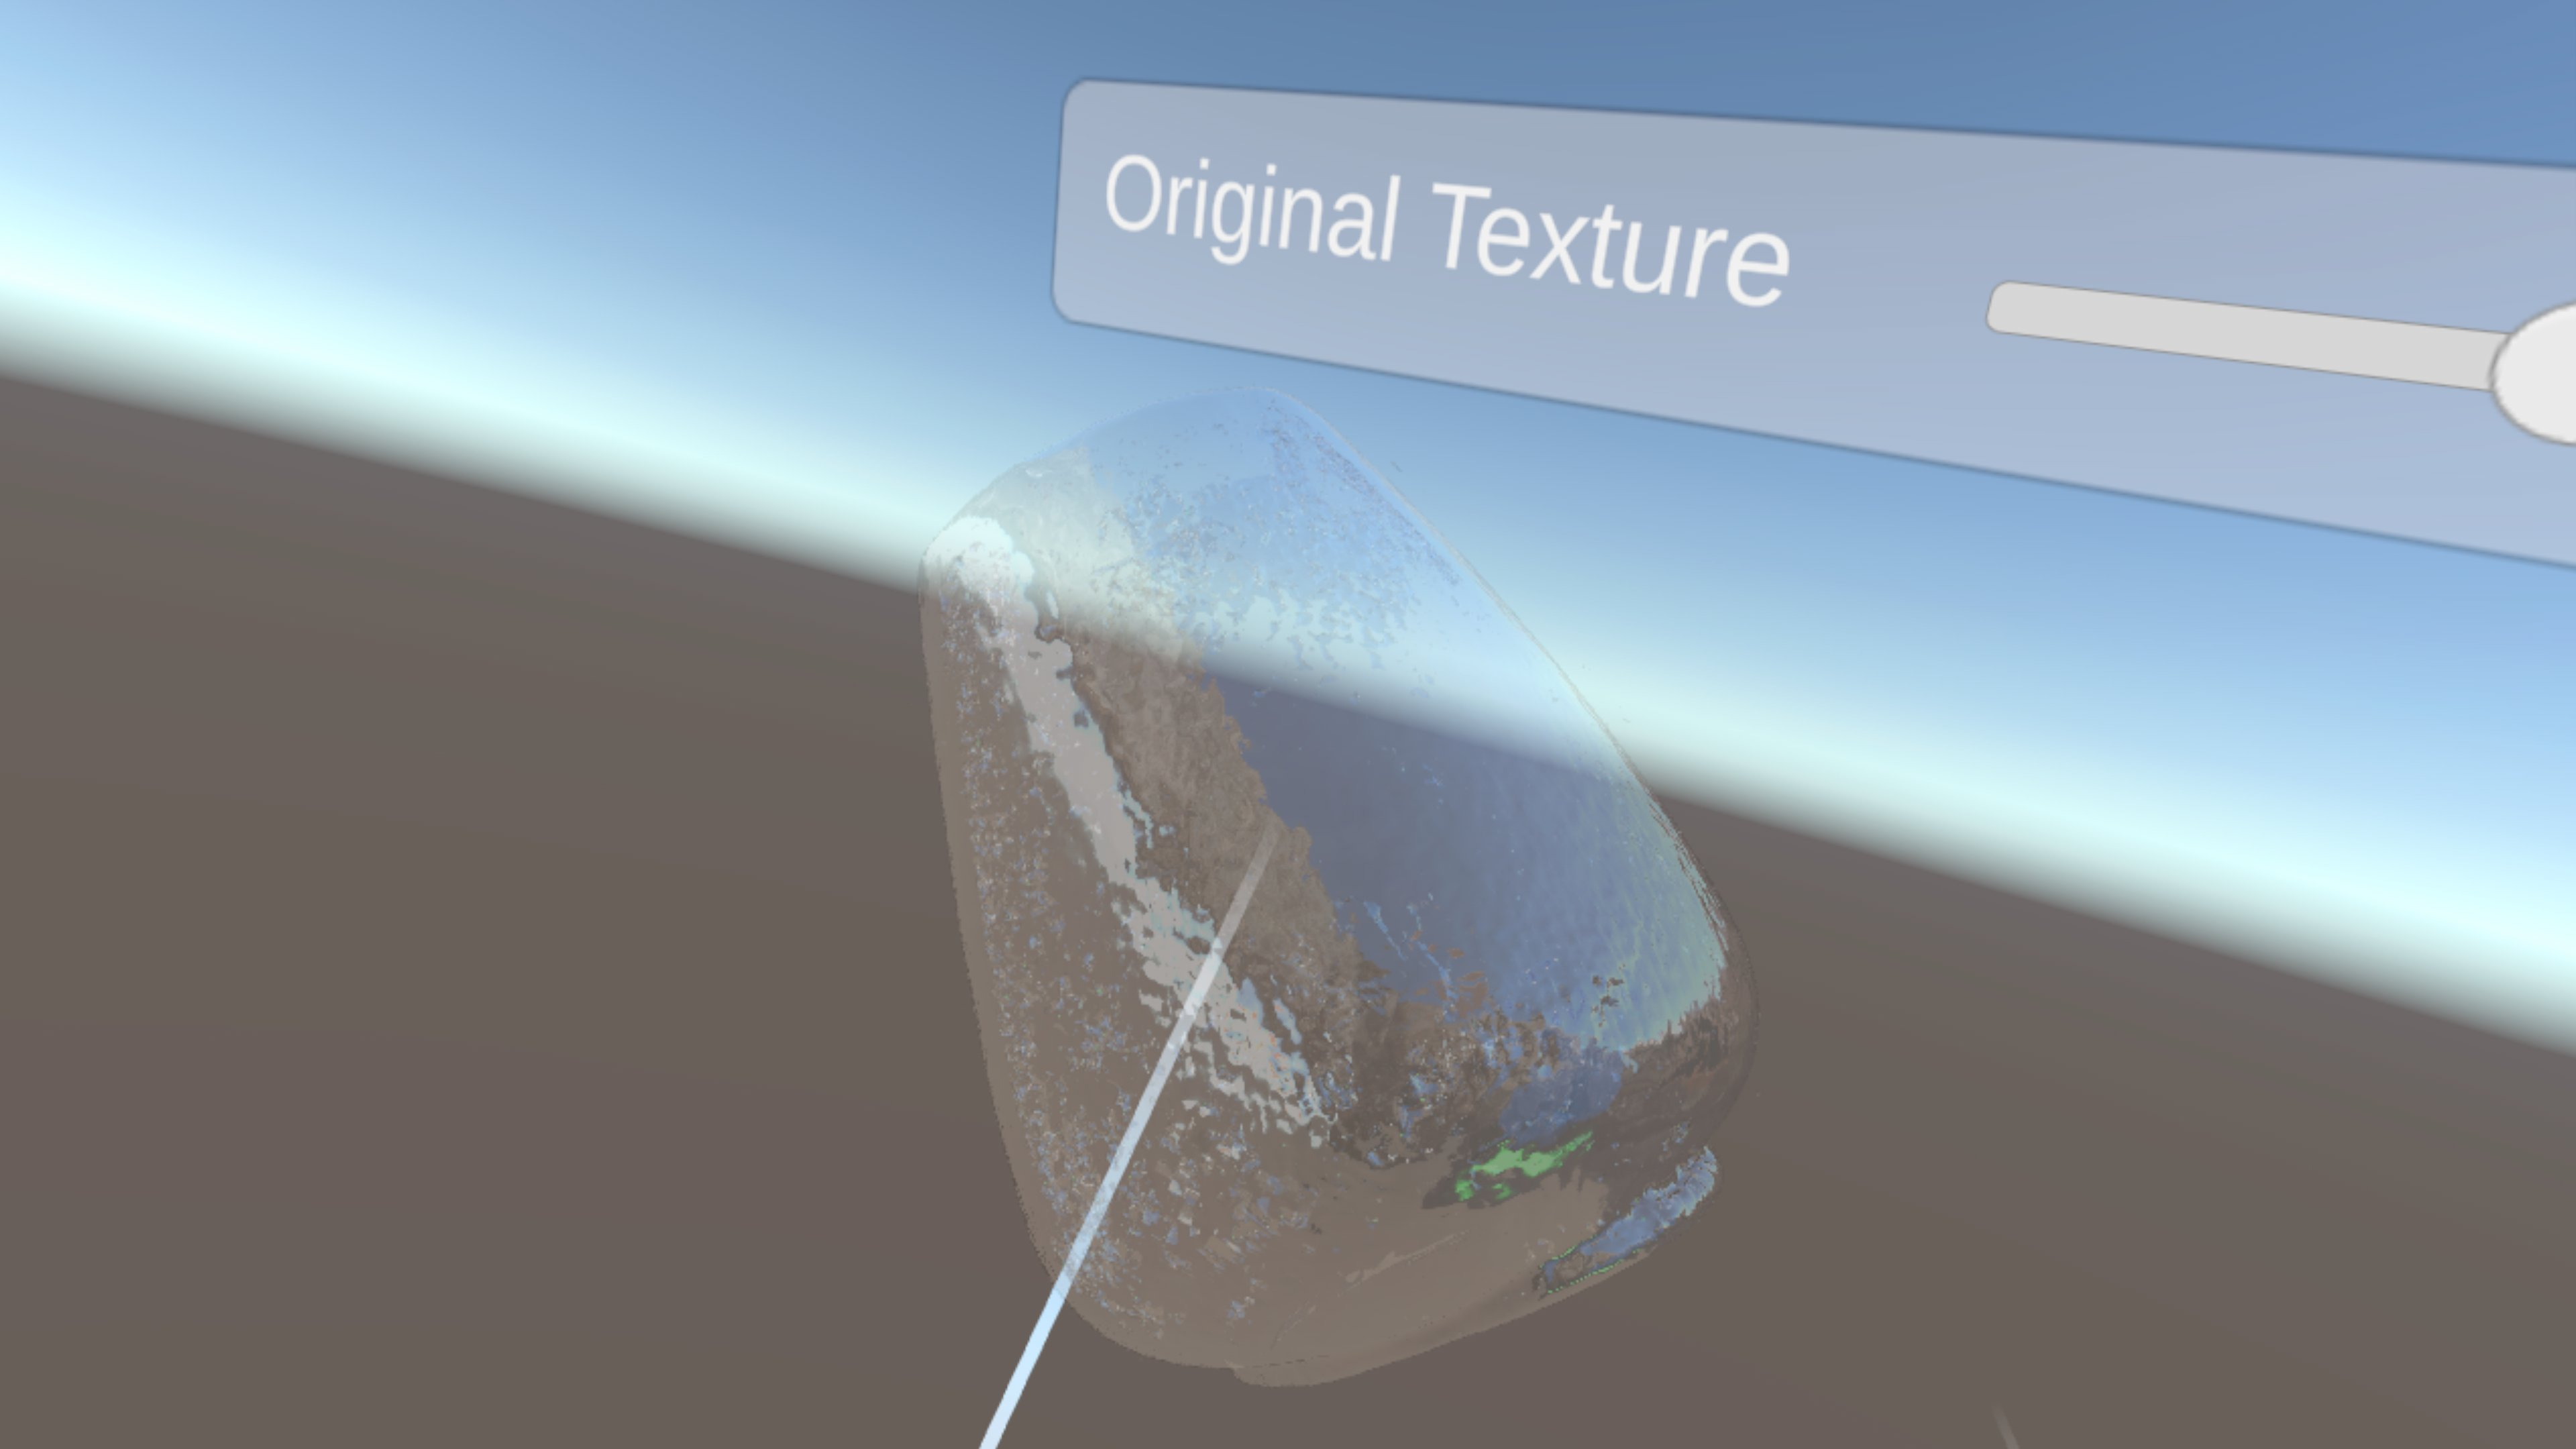
\includegraphics[width=0.8\textwidth]{Implementation/glass_1}
    \caption{Glass Texture of Object with ID 21684.}
    \label{fig:glass1}
\end{figure}


% \begin{figure}[h!]
%     \centering
%     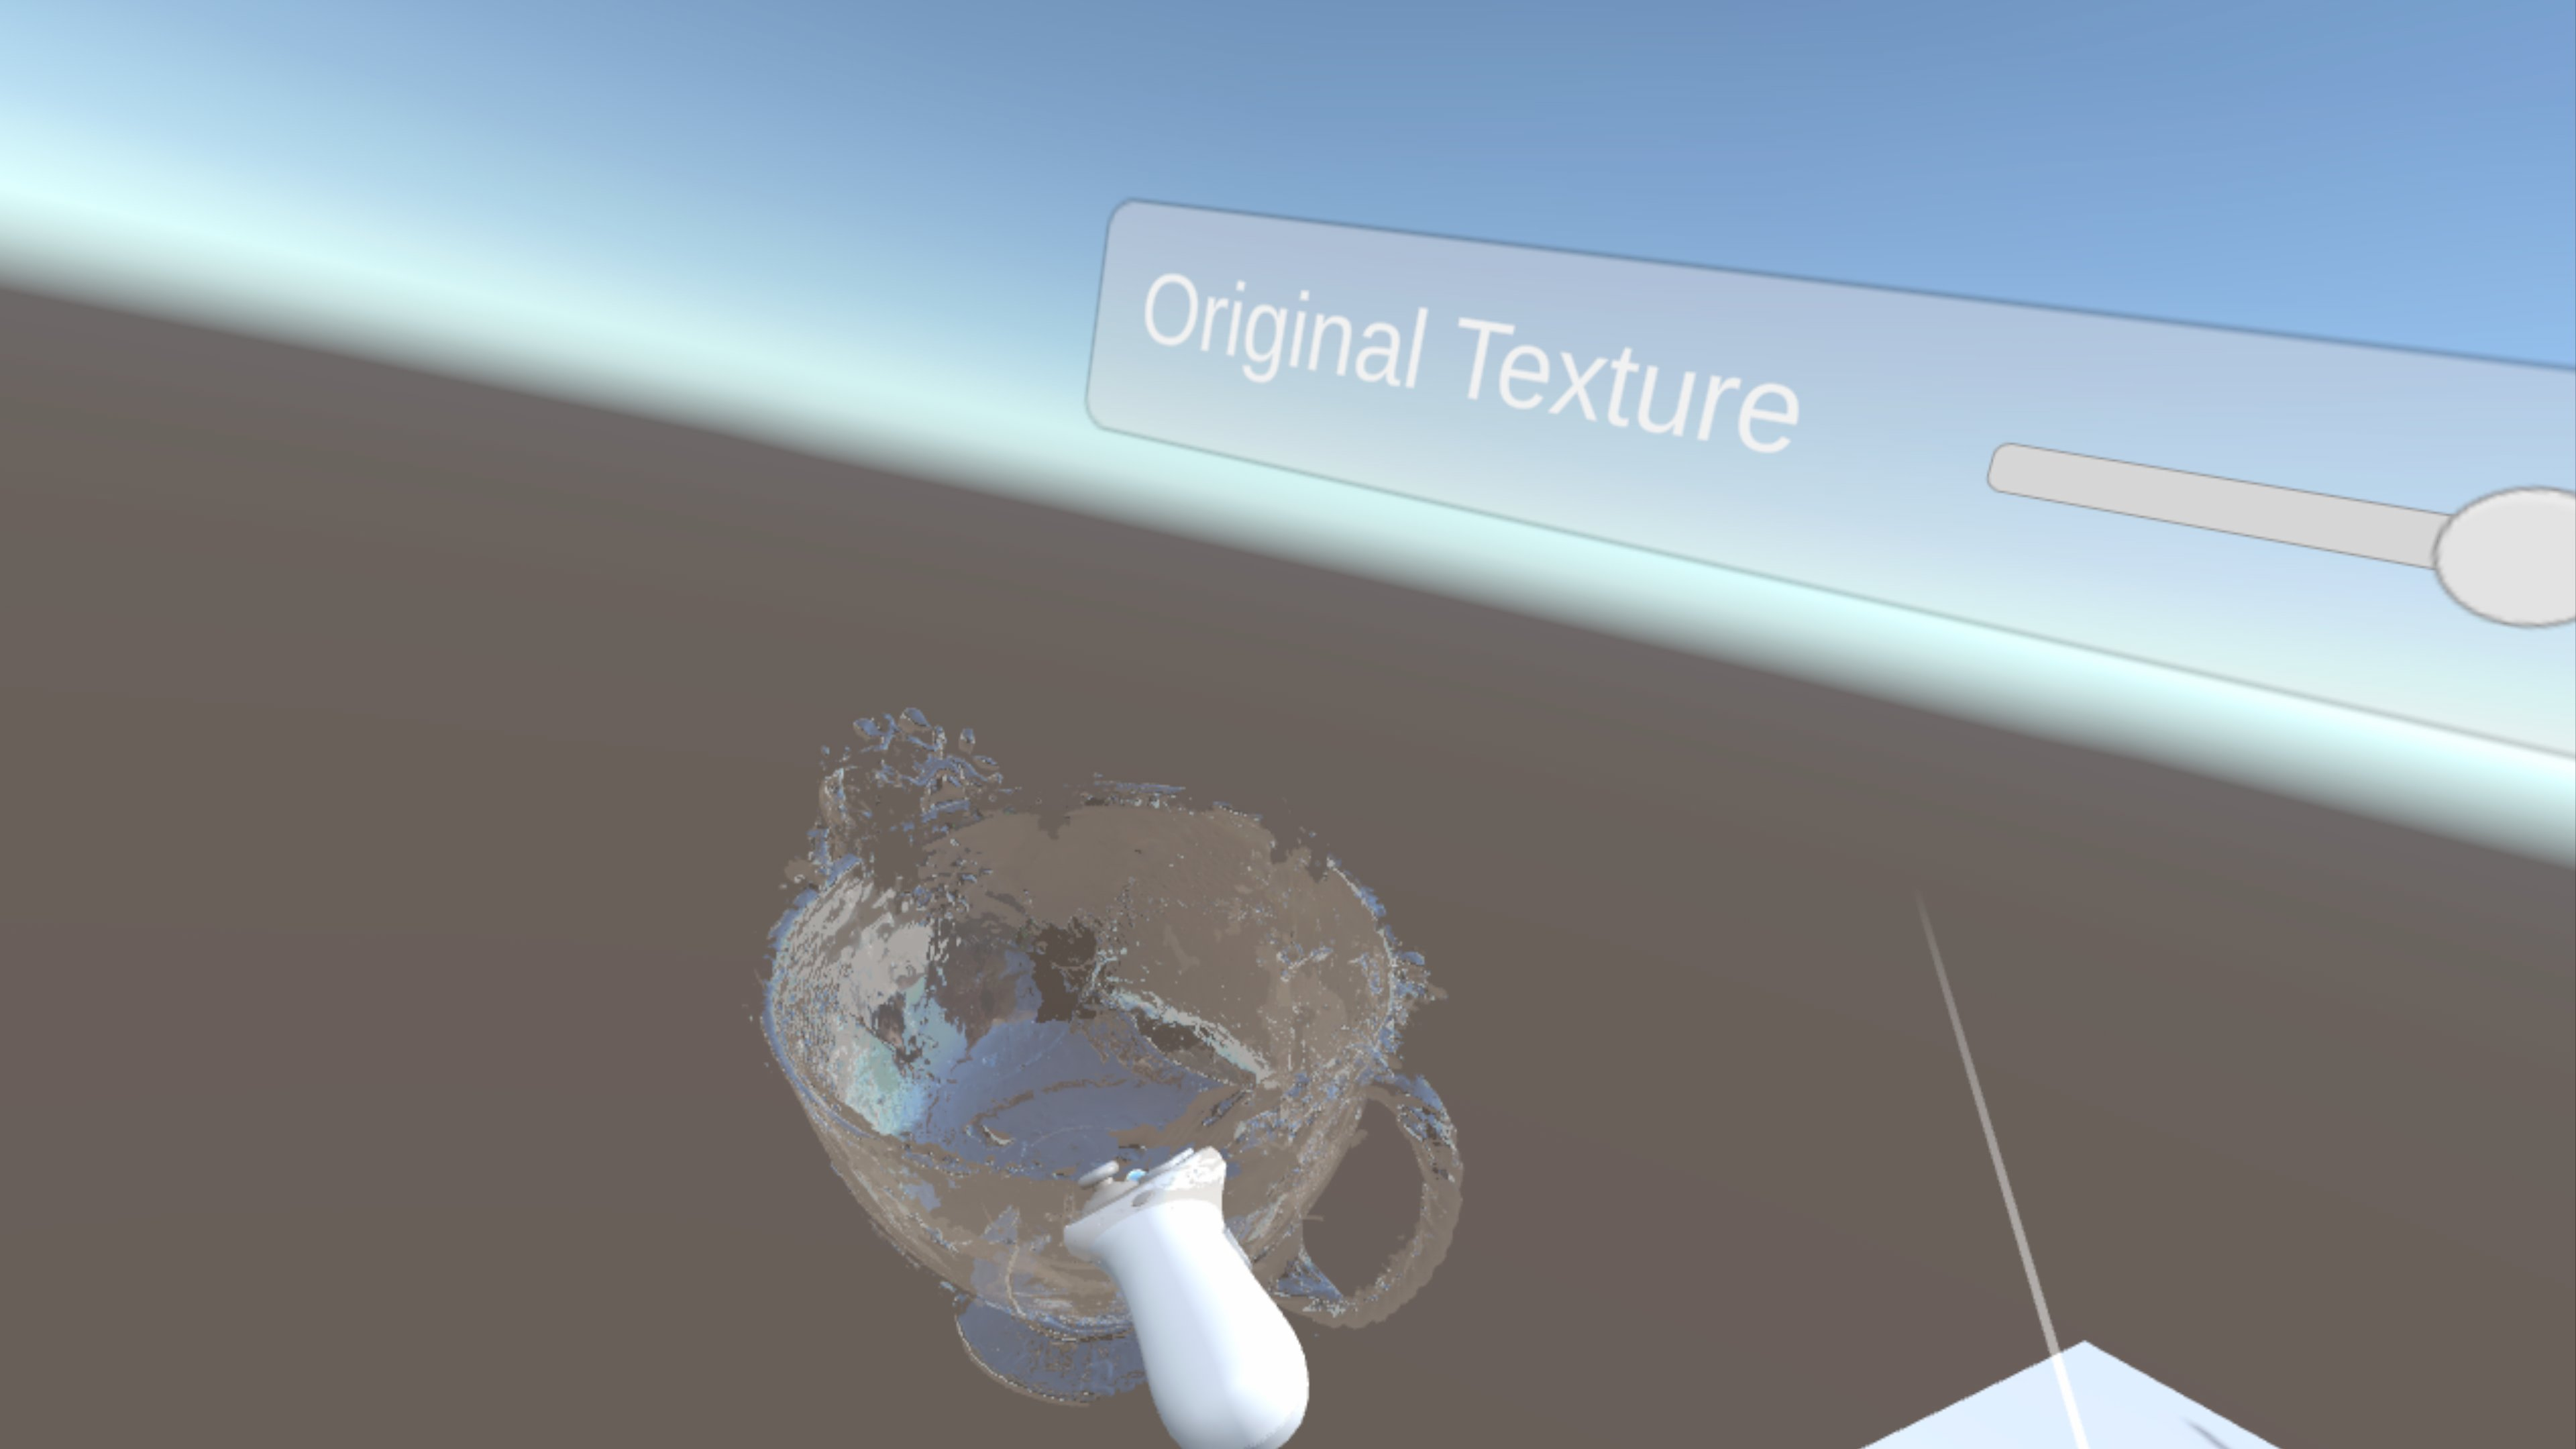
\includegraphics[width=0.8\textwidth]{Implementation/glass_2}
%     \caption{Glass Texture of Object with ID 21676.}
%     \label{fig:glass2}
% \end{figure}

\subsection{Generating the Funerary \gls{3D} Model}
\label{sec:build_model}

The funerary enclosure model was generated with the support of the photogrammetric survey and subsequently imported into the \textit{Sketchfab} viewer for intuitive interaction.
Within the grave, three open triangular areas were identified, containing the precious artefacts of the deceased, as shown in Figure~\ref{fig:model3} below.

This phase used the \textit{Agisoft Metashape} to stitch together photographs and capture the geometry, texture, and visual characteristics of the physical funerary structure.

The workflow began with the Align Photos operation, which produced 91,053 tie points. Then, a dense point cloud was generated to refine the level of detail, followed by the creation of a \gls{3D} mesh. The resulting model comprised 1,910,026 faces, for which a texture was mapped.
Finally, the model was exported in \texttt{.obj} format, and grouped with \texttt{.png} texture files, and imported into the Unity \gls{VR} environment.

\begin{figure}[h!]
    \centering
    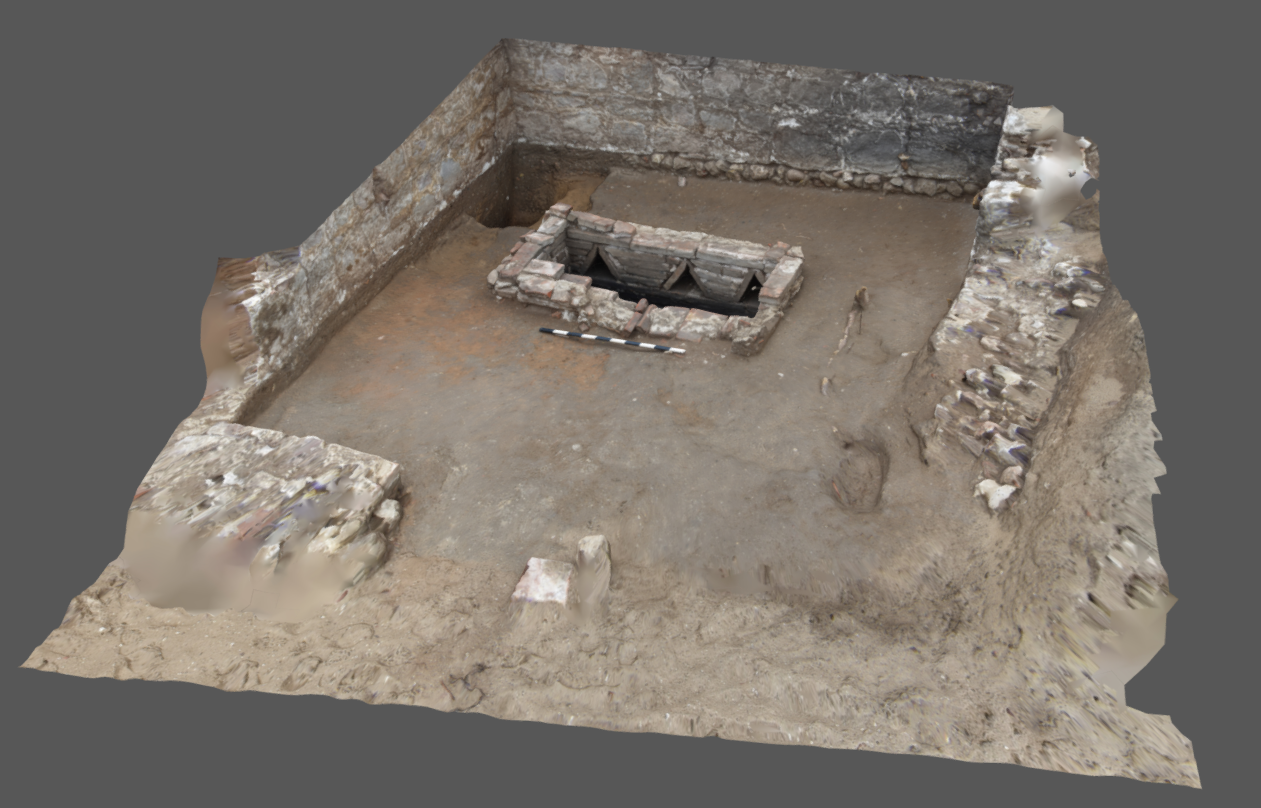
\includegraphics[width=0.7\textwidth]{model3}
    \caption{\gls{3D} Model in Sketchfab.}
    \label{fig:model3}
\end{figure}

\section{Testing and Debugging}
\label{sec:testing}

One of the most relevant features during the development phase on controller support was the \textbf{XR Device Simulator} included in XR Interaction Toolkit. 
This utility allowed for testing \gls{VR} interactions without the need for a physical \gls{HMD}. 
It simulated input from \gls{VR} controllers using a standard mouse and keyboard. 
Despite its usefulness along this dissertation, it's important to note that certain interactions did not behave identically compared to testing with the actual headset.

During the development, the functionalities within the environment were tested in real-time using the \emph{MetaLink} app. However, when connected via Wi-Fi, the environment did not load correctly. This issue was resolved by employing a wired connection.

Additionally, debugging was performed with the Visual Studio debugger and Android Debug Bridge (adb). 
This second tool enabled a in-depth troubleshooting and the identification of issues in the interaction with the headset by accessing detailed system logs through the \texttt{adb logcat} command. The logs proved useful for tracing errors and understanding their source during testing.


\section{Conclusions}
\label{sec:impl_discussion}

The implementation began with the generation of the funerary enclosure model.
Subsequently, the map was integrated into the Unity environment, initially empty.
Then, the model of the funerary enclosure was positioned on the map.
Following, the functionalities were implemented, such as \gls{3D} model visualization and map navigation, in accordance with the requirements outlined in Section \ref{sec:requirements}. 
Users can also grab objects, and interact with panel menus that displayed data retrieved from the database. 
A database was created to store significant data, including artefact and excavation data, with updates during development when needed. For interaction inside the tomb, two glass objects were chosen as the primary focus.

To enable communication between Unity and the database, a backend was implemented. Unity sent requests to the backend, which then queried the database and returned the requested information. 
A \emph{dropdown menu} was created in the \gls{VE} to fulfill requirement "Contextual Overlay", allowing the user to select an artefact ID and access the corresponding textual and visual data. 
Two request types were defined: (i) retrieval of all available ID from the "object" table, and (ii) retrieval of associated textual and image data, combining information from the "object" and "object\_intervention" tables.
For the layer toggle requirement, a photograph of the actual site was integrated, providing a stronger sense of presence for the user. Perspective switching was supported through photographs provided by specialists of the funerary enclosure architecture materials. 

The artefact reconstruction requirement was simplified: instead of reconstructing fragmented models, an illustration of the original object texture was simulated through the \emph{Object Slider} functionality.
As a result, users could enter the tomb and experience an immersive interaction with two glass relics, fulfilling the requirements of the \gls{VR} environment. Additional points of interest were distributed across the map to enrich the user experience.

Each functionality was tested individually, which was useful for correcting errors. After implementation, system testing evaluated the usability of the functionalities implemented to accomplish these requirements.